% This is samplepaper.tex, a sample chapter demonstrating the
% LLNCS macro package for Springer Computer Science proceedings;
% Version 2.21 of 2022/01/12
%
\documentclass[runningheads]{llncs}
\usepackage{tabularx}
%
\usepackage[T1]{fontenc}
\usepackage{listings}
% T1 fonts will be used to generate the final print and online PDFs,
% so please use T1 fonts in your manuscript whenever possible.
% Other font encondings may result in incorrect characters.
%
\usepackage{graphicx}
% Used for displaying a sample figure. If possible, figure files should
% be included in EPS format.
%
% If you use the hyperref package, please uncomment the following two lines
% to display URLs in blue roman font according to Springer's eBook style:
%\usepackage{color}
%\renewcommand\UrlFont{\color{blue}\rmfamily}
%\urlstyle{rm}
%
\begin{document}
%
\title{Finding the Closest OSM Objects to me}
%
%\titlerunning{Abbreviated paper title}
% If the paper title is too long for the running head, you can set
% an abbreviated paper title here
%
\author{Tyler Kelsey}
%
\institute{Albert-Ludwigs-Universität Freiburg, Freiburg im Breisgau, Germany}
\maketitle              % typeset the header of the contribution
%
\section{Introduction}
OpenStreetMap (or OSM) is an open source, easy-to-contribute map with the goal of being a free, editable map of the whole world made by people like me and you. This makes it very easy to access mapping data, as there are many APIs, as well as downloadable area maps.

OpenStreetMap works with a tagging system. Elements are given geometry (e.g. 'Node' or 'Way') which represent the physical location of the elements in coordinate form. OSM also supports a free format text tagging system, where users can add any tag they like. A tag consists of two elements, a 'key' and a 'value'. The key roughly corresponds to the overarching category of the tag, e.g. 'amenity', or as we use later in the report, 'healthcare'. The value then specifies exactly what object is it, e.g. 'bar' or 'psychotherapist'. Any number of tags can be added to an object. Even streets are objects in OSM.

In this report we are interested in extracting OSM objects, then formatting them using a CLI tool or Plotting them using matplotlib. As a bonus, we will use web-scraped phone numbers to show the potential of data merging to get more accurate, reliable data. Understanding the inner workings of OSM is not important for this report. 

To extract the data, we use the python library Pyrosm, as it suits the requirements perfectly. Alternatively, we could use the Overpass Turbo Rest API, but using Pyrosm is much faster when handling large datasets, as it downloads the entire region into a temporary folder and extracts a pandas dataframe, which is efficient to filter over and extract relevant elements. Large regions such as Baden-Württemberg would not be possible if we had used a Rest API.

In the following part of the report, we will talk about the two main contributions:

First, we will focus on the implementation of the code, including filling the dataframe, filtering the data, using a formatting LLM, and webscraping additional phone numbers.

Then, we will focus on plotting the data using jupyter notebook and printing the data using a CLI, along with hurdles in data manipulation that produced rogue errors.

\section{Implementation}
As the jupyter notebook implementation lays the code out in a very natural, front-to-back structure we will describe the relevant code parts using that structure.

First, we have to locate the user. Using the Nominatim library from geopy allows us to input free-form text and translate that into a (mostly) standardized address.

Then, we download the PBF (Protocalbuffer Binary Format, an efficient file format for OSM data) data for the smallest OSM region we can find that the user is located in. We also use the Haversine formula to properly handle the earth being round while calculating the size of the bounding box.

We then filter all elements into the dataframe. This filters out all irrelevant elements, including ones not in the bounding box, and ones not containing the relevant OSM tag. 

From here we have our relevant data. Here, a problem arises. Looking at, for example, the phone numbers of our elements, we can see that OSM data isn't very complete or reliable. Sometimes, the coordinates are missing from the elements. The reason they can still be plotted is that their geometry tag contains a shape consisting of coordinates. Most likely, Pyrosm fails to convert them to coordinates when filling the dataframe. This can be fixed by extracting the coordinates of elements that are missing from the geometry and overwriting the coordinate columns in the dataframe. The bigger problem is that OSM mappers rarely care to update phone numbers, or even add them in the first place. We can solve issues like these using data merging. To get a second dataset, we use a small LLM using ollama to translate the OSM tag into German. We created a suitable system prompt, and after testing, realized that this is perfect use case for a small local LLM, as it's fast and accurate. By using the translated key and the names of the elements extracted from our dataframe we get the URLs of the websites of our elements. By web scraping these sites we are able to extract current phone numbers using a custom regex.
\begin{lstlisting}
target_scraped_phones = []

for url in target_urls:
    if url == "":
        target_scraped_phones.append("Phone not specified")
        continue
    html = fetch_html(url)
    try:
        unsanitized_phone = re.search(r'(\
        ((\+49)( (\(0\)) )?| \ # Look for +49 or +49 (0)
        0\d{3,4}[\/ ])       \ # or look for 0 and 3-4 digits
        [^#%:;{},.\d\n]{0,3} \ # Allow 0-3 special characters
        (\d{3,10})           \ # Require 3-10 digits
        [^#%:;{},.\d\n\w]?   \ # Allow one special character
        (\d{3,7}) m          \ # Require 3-7 digits
        [^#%:;{},.\d\n\w]?   \ # Allow one special character
        (\d{2,4})?           \ # Allow 2-4 digits
        [^#%:;{},.\d\n\w]?   \ # Allow one special character
        (\d{0,2})?           \ # Allow 0-2 digits
        )', html).group(0)
    except:
        unsanitized_phone = ""
    phone = sanitize_phone(unsanitized_phone)
    target_scraped_phones.append(phone)
\end{lstlisting}
Finally we overwrite the old phone numbers with the web scraped ones, where applicable. This means that, in our sample query, 4/13 phone numbers were correct. Web scraping found 6/13, and after merging we end with 9/13 phone numbers, which is a solid increase. Limitations to the web scraping implementation are wrong websites, the phone number being hidden behind a separate link, and very strangely formatted phone numbers. Those limitations are why we could only extract 6/13 phone numbers.

\section{Plotting and CLI}
To visualize our program, we can use a test input and see what plots are created.

\begin{table}[]
    \centering
    \begin{tabular}{c | l}
        tag &  healthcare=psychotherapist \\
        location & Lehener str. 90 Freiburg
    \end{tabular}
    \bigskip
    \caption{Example user input}
    \label{tab:my_label}
\end{table}

The program accepts radius if given, but will default to 3 km. From now on, the OSM elements that have this specific tag will be called PoIs (Points of Interest). An additional feature of our program is that not only entire tags, but also keys without values are also supported. Using GeoPandas, which plots mapping data seamlessly into matplotlib, we get a plot with the x and y-axis representing the longitude and latitude, respectfully (Figure 1).


To aid the visuals, first all buildings are plotted to create a recognizable map, then the PoIs are plotted on top. 

One problem that arises from this method is that PoIs that are nodes are represented as scatterplot dots, while PoIs that are polygons are drawn as buildings, as seen (Figure 1). This makes small buildings hard to see if a large radius is selected, but is useful when looking at keys like 'landuse' or 'agriculture'. As a compromise, in Figure 2, where we narrow the PoIs down to the value 'psychotherapist', we edit the dataframe to change all polygons into nodes.



By summing the types of healthcare over the dataframe we can extract more useful information. Here 'doctor' usually refers to an unspecialized doctor, in German 'Hausarzt'. With this data we can create a pie chart (Figure 3).


The last plot can be created to display the final output in plot form: Labeling the data points, and sorting them by distance on the x-axis (Figure 4).


For the CLI tool the code was refactored in a more traditional fashion, with each step separated into functions to aid the comprehension of the 'main' code block. The big addition of this part of the program is using the argparse, logging, tqdm and subprocess modules. The basic CLI interface was built using argparse, allowing the user to select different parameters along with a few useful options, namely '--radius', '--map', and '--noscrape', manually controlling the radius, OSM map, and web scraping, respectfully. 

Logging is used to communicate with the user about the current step to program is on, along with allowing us to throw exceptions to the terminal. This is important as the successful execution of this program is inherently unprovable without solving the problem oneself: For instance, to tell if the program will fail due to not finding a single PoI in the radius, one would have to find out if there is atleast one PoI in the radius, which again is the basis of what our program does. Using logging lets us throw error messages in such cases, preventing the user from being confronted with confusing python error messages.

Tqdm is used to provide a loading bar to the user during the web scraping step. Due to the sorting of elements being extracted away from us by Pyrosm, it isn't possible to use a loading bar in that step.

Subprocess is used to output the final tabular to the user. The output is sorted by distance and is displayed to the user in this format:

\begin{table}[]
    \centering
    \begin{tabular}{c|c|c}
        distance & Name & Phone \\
        \hline
        0.74 km & Andreas Hansen & +4976115519658 \\
        0.79 km & Praxis für Systemische Therapie & 0 1601491448 \\
        ... & ... & ...
    \end{tabular}
    \bigskip
    \caption{Example output of the CLI tool}
    \label{tab:my_label}
\end{table}

\section{Most Interesting Results}
Due to the nature of OSM, anything that can be tagged will be tagged, unlike Google maps. This means that military installations that the public has found are listed, while Google often has characteristic 'gray spots' in such locations. Using our tool reveals information about such areas, such as locations, and, with a few additional lines of code, the count of the different installations.

Similarly interesting is the share of religion in different regions of Germany. If we compare Munich with Bremen, we can see that the data inferes that Bayern is more christian than Bremen, or atleast there is a greater share of christian PoIs in Munich than in Bremen.

\section{Conclusion}
While this project started out with the question "How can we use OSM data to generate plots and list PoIs", the addition of data merging using a web scraper and a self-contained CLI tool round out the project improved the usability of this project drastically. There are many areas of possible improvement, such as tags such as 'phone number' being able to be specified by the user, but that would be too much for the scope of this project. 

Some of the features of this program are possible on websites like Overpass Turbo, but this program allows local execution and viewing, opening the door to further experimentation and usage in other projects.
General limitations arise from the use of user-generated data. Wherever users are responsible for adding data, mistakes are bound to happen. We've seen that OSM data is only moderately reliable, yet another aspect is the way we handle mapping data. Addresses are not standardized between countries, which is one of the biggest reasons this tool is limited to Germany. Regional mapping data is also not available everywhere, for example the only italian map currently available is a map of the entirety of Italy, which requires more then 32 GBs of memory to use. Such is also the reason we always attempt to find the smallest possible map containing our location. On low-memory laptops even states such as Bayern could be difficult to process. Borders also are inherently difficult, as loading multiple maps when in a border region would require too much memory.

Overall, we can see that the goal was reached. We found that OSM data is moderately unreliable, yet can be augmented with data merging, and that OSM datasets are computationally complex to use. In the future, an interesting project could be sorting OSM data into more efficient data structures, allowing quick retrieval of elements in specific locations or by tag.

        

\begin{table}
\caption{Topics}
\begin{tabularx}{\textwidth}{ l  X }
Topics \\
\hline
Linux & Made using linux. Otherwise nothing to report.\\
Emacs & Not used.\\
Terminal & Has CLI functionality (see section 3). \\
Git & We used git as a version control system, otherwise nothing to report.\\
Modal editors & Not used.\\
python & Both parts of the program were written in solely in python, making extensive use of the automation libraries argparse, subprocess and logging. \\
vscode & VSCode was used for the seamless Jupyter Notebook integration, although it is not necessary to display the plots. \\
plots & We plotted data of the PoIs into multiple plots using GeoPandas and matplotlib. \\
\LaTeX & Was used to create this report. Nothing else to report. \\
LLMs & We created a system prompt for an Ollama LLM to translate the OSM key or value into german to enable more precise web scraping. 
\end{tabularx}
\end{table}

\begin{figure}
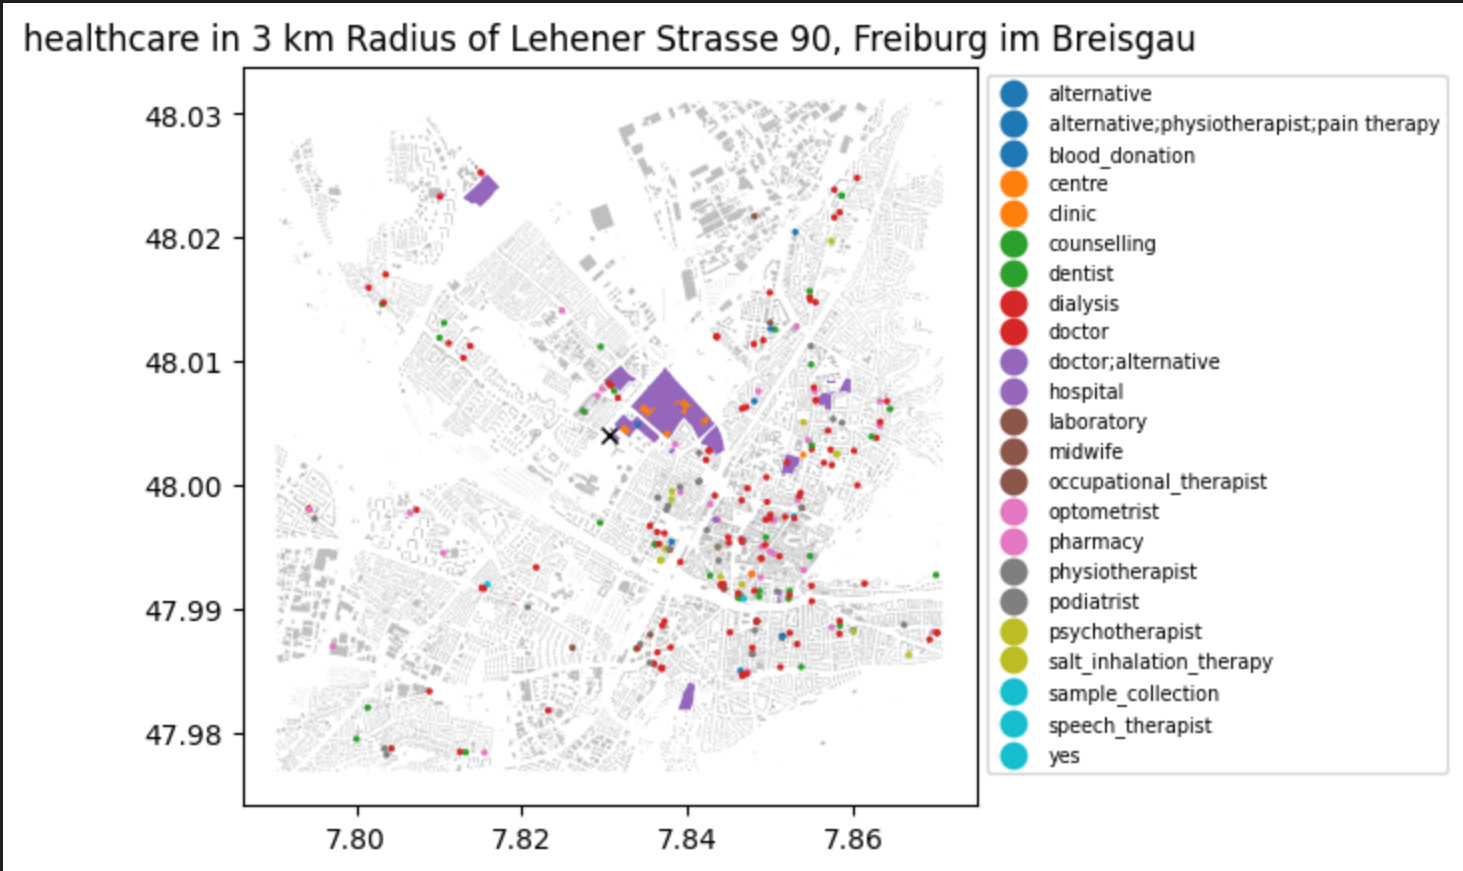
\includegraphics[width=\textwidth]{../images/freiburg_healthcare}
\caption{All healthcare in radius of the user} \label{fig1}
\end{figure}


\begin{figure}
    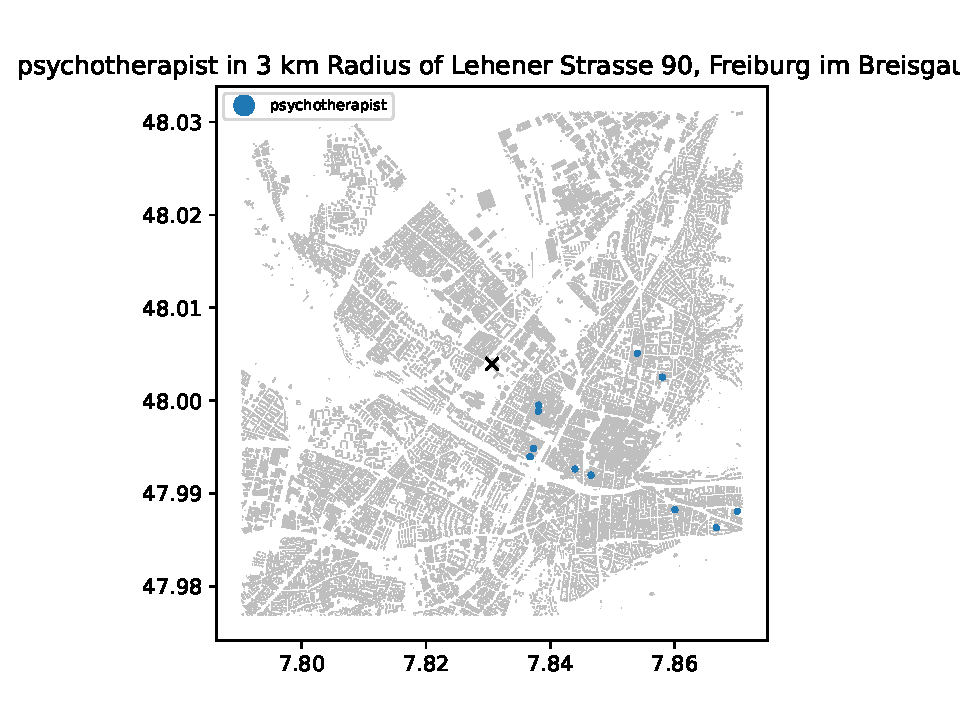
\includegraphics[width=\textwidth]{../images/freiburg_psychotherapists}
    \caption{Psychotherapists in radius of the user} \label{fig2}
    \end{figure}

\begin{figure}
    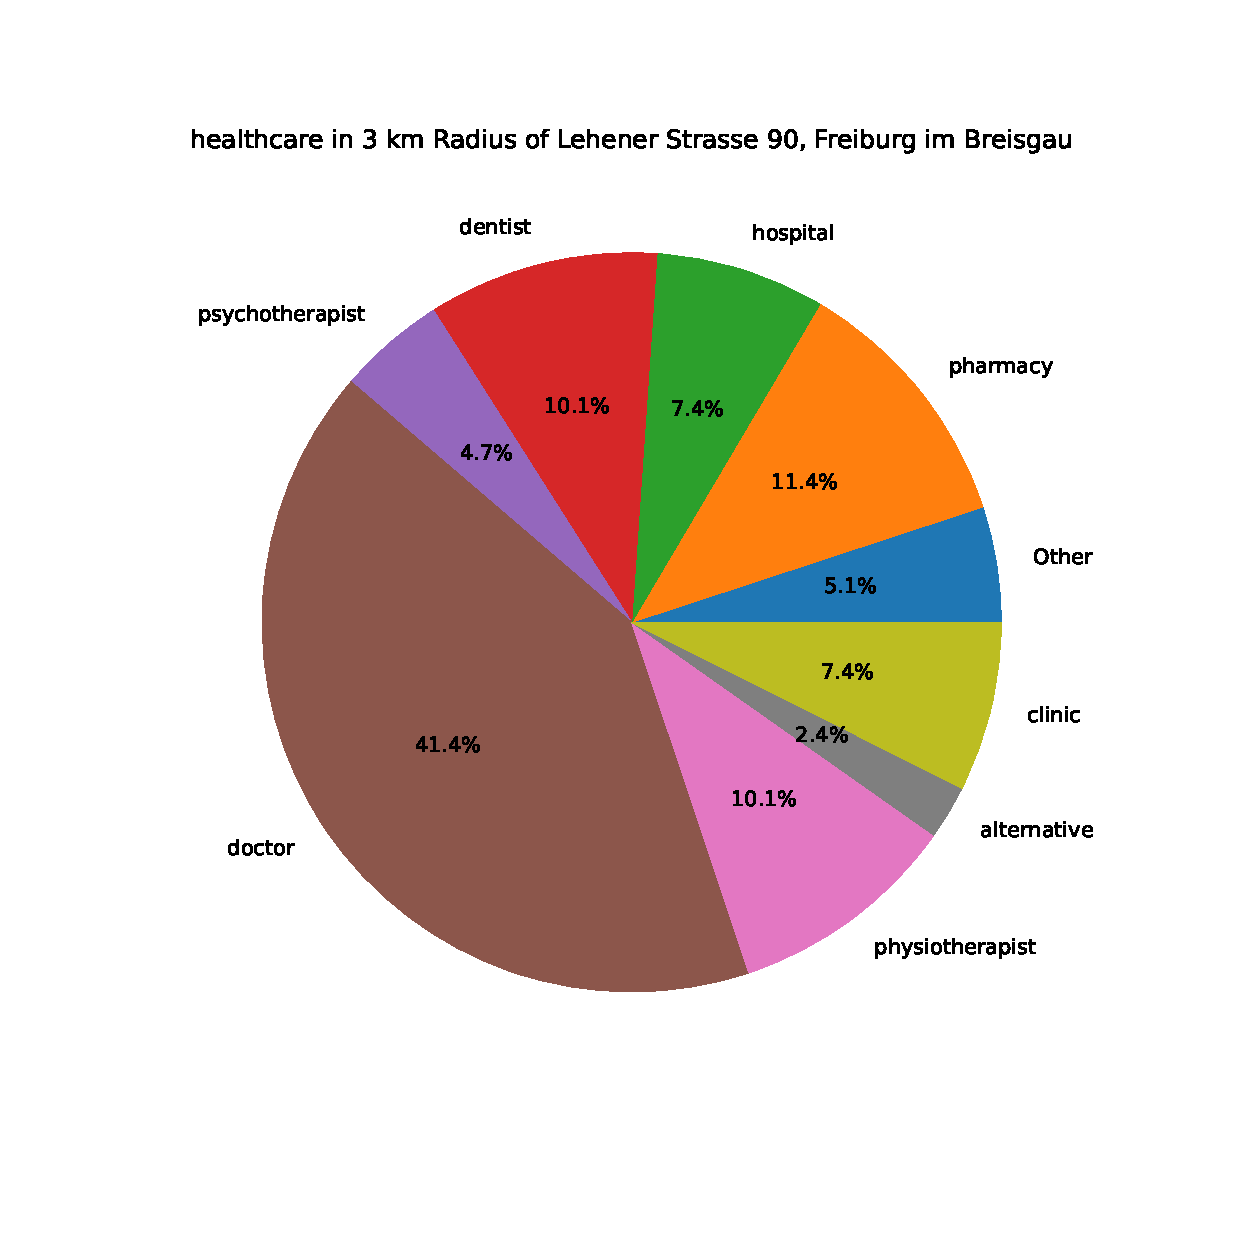
\includegraphics[width=\textwidth]{../images/freiburg_healthcare_pie}
    \caption{Types of healthcare in radius of user} \label{fig3}
    \end{figure}

\begin{figure}
    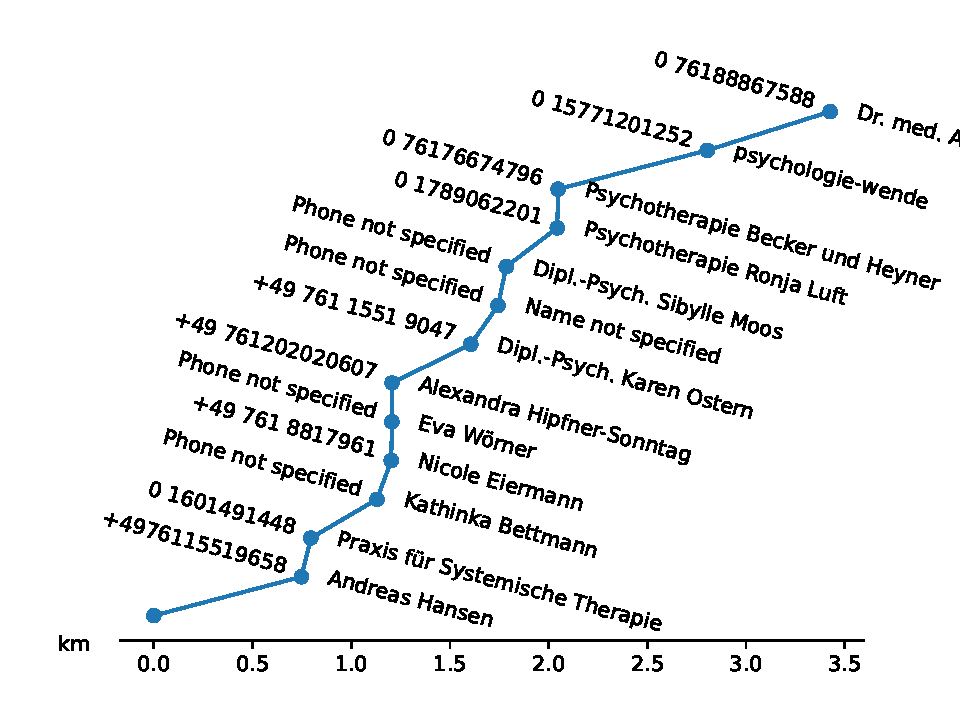
\includegraphics[width=\textwidth]{../images/freiburg_psychotherapists_distance}
    \caption{CLI output plotted} \label{fig4}
    \end{figure}

\end{document}
